%% abtex2-modelo-trabalho-academico.tex, v-1.9.6 laurocesar
%% Copyright 2012-2016 by abnTeX2 group at http://www.abntex.net.br/ 
%%
%% This work may be distributed and/or modified under the
%% conditions of the LaTeX Project Public License, either version 1.3
%% of this license or (at your option) any later version.
%% The latest version of this license is in
%%   http://www.latex-project.org/lppl.txt
%% and version 1.3 or later is part of all distributions of LaTeX
%% version 2005/12/01 or later.
%%
%% This work has the L PPL maintenance status `maintained'.
%% 
%% The Current Maintainer of this work is the abnTeX2 team, led
%% by Lauro César Araujo. Further information are available on 
%% http://www.abntex.net.br/
%%
%% This work consists of the files abntex2-modelo-trabalho-academico.tex,
%% abntex2-modelo-include-comandos and abntex2-modelo-references.bib

% ------------------------------------------------------------------------
% ------------------------------------------------------------------------
% abnTeX2: Modelo de Trabalho Academico (tese de doutorado, dissertacao de
% mestrado e trabalhos monograficos em geral) em conformidade com 
% ABNT NBR 14724:2011: Informacao e documentacao - Trabalhos academicos -
% Apresentacao
% ------------------------------------------------------------------------
% ------------------------------------------------------------------------
% Personalização para o modelo Udesc 2020 7. ed. revisada e modificada
% MANUAL_2020_09_07_1599489825065_12510.pdf
% Autor: Felipe Joel Zimann (felipezimann@hotmail.com)
% Data: 02/12/2020 v1.0
% Data: 13/02/2021 v1.0.1 alterado tamanho numeração da página para 10pt
% ------------------------------------------------------------------------
% ------------------------------------------------------------------------

\documentclass[
	12pt,				% tamanho da fonte
	openright,			% capítulos começam em pág ímpar (insere página vazia caso preciso)
	oneside,			% para impressão em recto e verso (twoside). Oposto a (oneside)
	a4paper,			% tamanho do papel. 
	chapter=TITLE,		% títulos de capítulos convertidos em letras maiúsculas
	section=TITLE,		% títulos de seções convertidos em letras maiúsculas
	sumario=abnt-6027-2012,
	english,			% idioma adicional para hifenização
	brazil,				% o último idioma é o principal do documento
	fleqn,				% equações alinhadas a esquerda (UDESC/CCT)+
	]{abntex2}

% ----------------------------------------------------------
% Pacotes básicos 
% ----------------------------------------------------------
\usepackage{amsmath}							% Pacote matemático
\usepackage{amssymb}							% Pacote matemático
\usepackage{amsfonts}							% Pacote matemático	
\usepackage{mathptmx} 							% Usa a fonte Times New Roman	 (UDESC/CCT)
\usepackage[T1]{fontenc}						% Selecao de codigos de fonte.
\usepackage[utf8]{inputenc}						% Codificacao do documento (conversão automática dos acentos)
\usepackage{lastpage}							% Usado pela Ficha catalográfica
\usepackage{indentfirst}						% Indenta o primeiro parágrafo de cada seção.
\usepackage[dvipsnames,table]{xcolor}			% Controle das cores
\usepackage{graphicx}							% Inclusão de gráficos
\usepackage{microtype} 							% para melhorias de justificação
\usepackage[brazilian,hyperpageref]{backref}	% Paginas com as citações na bibl
\usepackage[alf,abnt-emphasize=bf,abnt-full-initials=yes,abnt-etal-list=0]{abntex2cite}					% Citações padrão ABNT
\usepackage{adjustbox}							% Pacote de ajuste de boxes
\usepackage{subcaption}							% Inclusão de Subfiguras e sublegendas		
\usepackage{enumitem}							% Personalização de listas
\usepackage{siunitx}							% Grandezas e unidades
\usepackage[section]{placeins}					% Manter as figuras delimitadas na respectiva seção com a opção [section]
\usepackage{multirow}							% Multi colunas nas tabelas
\usepackage{array,tabularx} 					% Pacotes de tabelas
\usepackage{booktabs}							% Pacote de tabela profissonal
\usepackage{rotating}							% Rotacionar figuras e tabelas
\usepackage{xfrac}								% Fazer frações n/d em linha
\usepackage{bm}									% Negrito em modo matemático
\usepackage{xstring}							% Manipulação de strings
\usepackage{pgfplots}							% Pacote de Gráficos
\usepackage{tikz}								% Pacote dSe Figuras
\usepackage{chngcntr}						% Pacte usado para deixar numeração de equações sequencial (UDESC/CCT)
\usepackage{tikz-3dplot} 
\usepackage{esint}

\usepackage{jlcode}

\counterwithout{equation}{chapter}
\usetikzlibrary{3d,perspective,shadings}



% fonte: https://latex.org/forum/viewtopic.php?t=15392

% Comando para deixar numeração das equações contínua (1), (2), (3)... ao invés de organizar por capítulos (1.1)(1.2)... (2.1)(2.2)
%\renewcommand{\theequation}{\arabic{equation}}

%\numberwithin{equation}{section}

% Cabecalho cabeçalho somente com numeração de página 10pt
\makepagestyle{PagNumReduzida}
\makeevenhead{PagNumReduzida}{\ABNTEXfontereduzida\thepage}{}{}
\makeoddhead{PagNumReduzida}{}{}{\ABNTEXfontereduzida\thepage}
%fonte: https://github.com/abntex/abntex2/wiki/HowToCustomizarCabecalhoRodape
%fonte: Manual memoir seção 7.3 pg. 111 pdf http://linorg.usp.br/CTAN/macros/latex/contrib/memoir/memman.pdf 

% Personalização das opções das listas
\setlist[itemize]{leftmargin=\parindent}

% Citação online --- MODIFICAR ---
\newcommand{\citeshort}[1]{\citeauthoronline{#1}~(\citeyear{#1})}

\newcommand{\me}[1]{Elaborado pelo autor (#1).}

% Configuração do pgfplots
\pgfplotsset{compat=newest} %compat=1.14
\pgfplotsset{plot coordinates/math parser=false} 
\newlength\figureheight 
\newlength\figurewidth 

% Libraries do TiKz
\usetikzlibrary{quotes,angles,arrows}
\usetikzlibrary{through,calc,math}
\usetikzlibrary{graphs,backgrounds,fit}
\usetikzlibrary{shapes,positioning,patterns,shadows}
\usetikzlibrary{decorations.pathreplacing}
\usetikzlibrary{shapes.geometric}
\usetikzlibrary{arrows.meta}
\usetikzlibrary{external}

%\tikzexternalize[]
%\tikzexternalenable
%\tikzexternalize
%\tikzexternaldisable
%\tikzset{external/force remake}
%\tikzexternalize[shell escape=-enable-write18]
% Personalização das legendas
\usepackage[format = plain, %hang
			justification = centering,
			labelsep = endash,
			singlelinecheck = false,
			skip = 6pt,
			listformat = simple]{caption}	

% Personalização das unidades
\sisetup{output-decimal-marker = {,}}
%\sisetup{exponent-product = \cdot, output-product = \cdot}
\sisetup{tight-spacing=true}
\sisetup{group-digits = false}

% Personalizações de tipo de colunas de tabelas
\newcolumntype{L}[1]{>{\raggedright\let\newline\\\arraybackslash\hspace{0pt}}m{#1}}
\newcolumntype{C}[1]{>{\centering\let\newline\\\arraybackslash\hspace{0pt}}m{#1}}
\newcolumntype{R}[1]{>{\raggedleft\let\newline\\\arraybackslash\hspace{0pt}}m{#1}}

% Personalizações de cores da UDESC
\definecolor{CapaAmareloUDESC}{RGB}{243,186,83}		% Especializacao
\definecolor{CapaVerdeUDESC}{RGB}{0,112,52}			% Mestrado
\definecolor{CapaVermelhoUDESC}{RGB}{171,35,21}		% Doutorado
\definecolor{CapaAzulUDESC}{RGB}{38,54,118} 		% Pós-Doutorado

% CONFIGURAÇÕES DE PACOTES
% Configurações do pacote backref
% Usado sem a opção hyperpageref de backref
\renewcommand{\backrefpagesname}{Citado na(s) página(s):~}
% Texto padrão antes do número das páginas
\renewcommand{\backref}{}
% Define os textos da citação
\renewcommand*{\backrefalt}[4]{
	\ifcase #1 %
	Nenhuma citação no texto.%
	\or
	Citado na página #2.%
	\else
	Citado #1 vezes nas páginas #2.%
	\fi}%

% alterando o aspecto da cor azul
%\definecolor{blue}{RGB}{41,5,195}

% informações do PDF
\makeatletter
\hypersetup{
	%pagebackref=true,
	pdftitle={\@title}, 
	pdfauthor={\@author},
	pdfsubject={\imprimirpreambulo},
	pdfcreator={LaTeX with abnTeX2},
	pdfkeywords={abnt}{latex}{abntex}{abntex2}{trabalho academico}, 
	colorlinks=true,       		% false: boxed links; true: colored links
	linkcolor=black,          	% color of internal links
	citecolor=black,        	% color of links to bibliography
	filecolor=black,      		% color of file links
	urlcolor=black,
	bookmarksdepth=4
}
\makeatother


\makeatletter
\newcommand{\includetikz}[1]{%
	\tikzsetnextfilename{#1}%
	\input{#1.tex}%
}
\makeatother

% ---
% Possibilita criação de Quadros e Lista de quadros.
% Ver https://github.com/abntex/abntex2/issues/176
%
\newcommand{\quadroname}{Quadro}
\newcommand{\listofquadrosname}{Lista de quadros}

\newfloat[chapter]{quadro}{loq}{\quadroname}
\newlistof{listofquadros}{loq}{\listofquadrosname}
\newlistentry{quadro}{loq}{0}

% configurações para atender às regras da ABNT
\setfloatadjustment{quadro}{\centering}
\counterwithout{quadro}{chapter}
\renewcommand{\cftquadroname}{\quadroname\space} 
\renewcommand*{\cftquadroaftersnum}{\hfill--\hfill}

\setfloatlocations{quadro}{hbtp} % Ver https://github.com/abntex/abntex2/issues/176
% ---


% Espaçamento depois do título
\setlength{\afterchapskip}{0.7\baselineskip}
% O tamanho do parágrafo é dado por:
\setlength{\parindent}{1.25cm}
% Controle do espaçamento entre um parágrafo e outro:
\setlength{\parskip}{0.0cm}  % tente também \onelineskip
%\SingleSpacing % Espaçamento simples 
\OnehalfSpacing % Espaçamento 1,5 (UDESC/CCT)
%\DoubleSpacing	% Espaçamento duplo

% ---
% Margens - NBR 14724/2011 - 5.1 Formato
% ---
\setlrmarginsandblock{3cm}{2cm}{*}
\setulmarginsandblock{3cm}{2cm}{*}
\checkandfixthelayout[fixed]
% ---


% To use externalize consider
%https://tex.stackexchange.com/questions/182783/tikzexternalize-not-compatible-with-miktex-2-9-abntex2-package
%Lauro Cesar digged into the problem until he came with a solution for me to test. And it Works!
%
%According to this link:
%
%The package calc changed the commands \setcounter and friends to be fragile. So you have to make them robust. The example below uses etoolbox with \robustify:
%
\usepackage{etoolbox}
\robustify\setcounter
\robustify\addtocounter
\robustify\setlength
\robustify\addtolength


%% How to silence memoir class warning against the use of caption package?
%% https://tex.stackexchange.com/questions/391993/how-to-silence-memoir-class-warning-against-the-use-of-caption-package
%\usepackage{silence}
%\WarningFilter*{memoir}{You are using the caption package with the memoir class}
%\WarningFilter*{Class memoir Warning}{You are using the caption package with the memoir class}

% --------------------------------------------------------
% INICIO DAS CUSTOMIZACOES PARA A UDESC
% --------------------------------------------------------

% --------------------------------------------------------
% Fontes padroes de part, chapter, section, subsection e subsubsection
% --------------------------------------------------------
% --- Chapter ---
\renewcommand{\ABNTEXchapterfont}{\fontseries{b}} %\bfseries
\renewcommand{\ABNTEXchapterfontsize}{\normalsize}
% --- Part ---
\renewcommand{\ABNTEXpartfont}{\ABNTEXchapterfont}
\renewcommand{\ABNTEXpartfontsize}{\LARGE}
% --- Section ---
\renewcommand{\ABNTEXsectionfont}{\normalfont}
\renewcommand{\ABNTEXsectionfontsize}{\normalsize}
% --- SubSection ---
\renewcommand{\ABNTEXsubsectionfont}{\fontseries{b}} %\bfseries
\renewcommand{\ABNTEXsubsectionfontsize}{\normalsize}
% --- SubSubSection ---
\renewcommand{\ABNTEXsubsubsectionfont}{\itshape}
\renewcommand{\ABNTEXsubsubsectionfontsize}{\normalsize}

\renewcommand{\ABNTEXsubsubsubsectionfont}{\normalfont}
\renewcommand{\ABNTEXsubsubsubsectionfontsize}{\normalsize}
% ---

% --------------------------------------------------------
% Fontes das entradas do sumario
% --------------------------------------------------------

\renewcommand{\cftpartfont}{\ABNTEXpartfont\selectfont}
\renewcommand{\cftpartpagefont}{\normalsize\selectfont}

\renewcommand{\cftchapterfont}{\ABNTEXchapterfont\selectfont}
\renewcommand{\cftchapterpagefont}{\normalsize\selectfont}

\renewcommand{\cftsectionfont}{\ABNTEXsectionfont\selectfont}
\renewcommand{\cftsectionpagefont}{\normalsize\selectfont}

\renewcommand{\cftsubsectionfont}{\ABNTEXsubsectionfont\selectfont}
\renewcommand{\cftsubsectionpagefont}{\normalsize\selectfont}

\renewcommand{\cftsubsubsectionfont}{\normalfont\itshape\selectfont}
\renewcommand{\cftsubsubsectionpagefont}{\normalsize\selectfont}

\renewcommand{\cftparagraphfont}{\normalfont\selectfont}
\renewcommand{\cftparagraphpagefont}{\normalsize\selectfont}

% --------------------------------------------------------
% Usando os pacotes hyperref, uppercase... 
% Para deixar a section do toc uppercase precisa de:
% --------------------------------------------------------
\usepackage{textcase}

\makeatletter

\let\oldcontentsline\contentsline
\def\contentsline#1#2{%
	\expandafter\ifx\csname l@#1\endcsname\l@section
	\expandafter\@firstoftwo
	\else
	\expandafter\@secondoftwo
	\fi
	{%
		\oldcontentsline{#1}{\MakeTextUppercase{#2}}%
	}{%
		\oldcontentsline{#1}{#2}%
	}%
}
\makeatother

% --------------------------------------------------------
% Renomenando as entradas de APÊNDICES E ANEXOS
% --------------------------------------------------------

\renewcommand{\apendicesname}{AP\^ENDICES}
\renewcommand{\anexosname}{ANEXOS}


% Manipulação de Strings
%\RequirePackage{xstring}

% Comando para inverter sobrenome e nome
\newcommand{\invertname}[1]{%
	\StrBehind{#1}{{}}, \StrBefore{#1}{{}}%
}%


% --------------------------------------------------------
% Alterando os estilos de Caption e Fonte
% --------------------------------------------------------
\makeatletter
% Define o comando \fonte que respeita as configurações de caption do memoir ou do caption
\renewcommand{\fonte}[2][\fontename]{%
	\M@gettitle{#2}%
	\memlegendinfo{#2}%
	\par
	\begingroup
	\@parboxrestore
	\if@minipage
	\@setminipage
	\fi
	\ABNTEXfontereduzida
	\configureseparator
	\captiondelim{\ABNTEXcaptionfontedelim}
	\@makecaption{#1}{\ignorespaces #2}\par
	\endgroup}


\captionstyle[\raggedright]{\raggedright}

\makeatother

\setlength{\cftbeforechapterskip}{0pt plus 0pt}
\renewcommand*{\insertchapterspace}{}

\newlength{\mylen}	% New length to use with spacing
\setlength{\mylen}{1pt}

\setlength{\cftbeforechapterskip}{\mylen}
\setlength{\cftbeforesectionskip}{\mylen}
\setlength{\cftbeforesubsectionskip}{\mylen}
\setlength{\cftbeforesubsubsectionskip}{\mylen}
\setlength{\cftbeforesubsubsubsectionskip}{\mylen}


% ---
% Ajuste das listas de abreviaturas e siglas ; e símbolos [Personalizada para UDESC com espaçamento 1,5]
% ---

% ---
% Redefinição da Lista de abreviaturas e siglas [Personalizada para UDESC com espaçamento 1,5]
\renewenvironment{siglas}{%
	\pretextualchapter{\listadesiglasname}
	\begin{symbols} 
		\setlength{\itemsep}{0pt}	% Ajuste para Espaçamento 1,5 (UDESC/CCT)
	}{% 
	\end{symbols}
	\cleardoublepage
}
% ---

% ---
% Redefinição da Lista de símbolos [Personalizada para UDESC com espaçamento 1,5]
\renewenvironment{simbolos}{%
	\pretextualchapter{\listadesimbolosname}
	\begin{symbols}
		\setlength{\itemsep}{0pt}	% Ajuste para Espaçamento 1,5 (UDESC/CCT)
	}{%
	\end{symbols}
	\cleardoublepage
}
% ---





% ---
% FIM DAS CUSTOMIZACOES PARA A  Universidade do Estado de Santa Catarina - UDESC/CCT
% ---





	% Incliu pacotes básicos 

% -----------------------------------------------------------------
% Você pode adicionar seus pacotes a partir desta linha;
% -----------------------------------------------------------------

%\usepackage[showframe,pass]{geometry}
%\usepackage[11,12]{pagesel}

% -----------------------------------------------------------------
% Informações de dados para CAPA e FOLHA DE ROSTO
% -----------------------------------------------------------------

\titulo{Título do Trabalho}%

\autor{Nome do Autor {}Sobrenome}%
\orientador{Nome do orientador{} Sobrenome}%
\coorientador{Nome do coorientador{} Sobrenome}%

% ATENÇÃO: O símbolo {} indica o sobrenome para a ficha catalográfica.
% Exemplo: Sherlock Holmes {}da Silva para sobrenomes compostos;
% Exemplo: Arnold Alois {}Schwarzenegger para sobrenome simples.

\instituicao{Universidade do Estado de Santa Catarina, Centro de Ciências Tecnológicas, Programa de Pós--Graduação em Engenharia Elétrica}%

%\tipotrabalho{Tese (Doutorado)}
\tipotrabalho{Dissertação (Mestrado)}

%\preambulo{Tese apresentada ao Programa de Pós--Graduação em Engenharia Elétrica do Centro de Ciências Tecnológicas da Universidade do Estado de Santa Catarina, como requisito parcial para a obtenção do grau de Doutor em Engenharia Elétrica.}

\preambulo{Dissertação apresentada ao Programa de Pós--Graduação em Engenharia Elétrica do Centro de Ciências Tecnológicas da Universidade do Estado de Santa Catarina, como requisito parcial para a obtenção do grau de Mestre em Engenharia Elétrica.}

\local{Joinville}%

\data{\the\year}%
% ---

% compila o indice
\makeindex

% -----------------------------------------------------------------
% Início do documento
% -----------------------------------------------------------------
\begin{document}

\selectlanguage{brazil}
\frenchspacing  % Retira espaço extra obsoleto entre as frases.

% -----------------------------------------------------------------
% ELEMENTOS PRÉ-TEXTUAIS
% -----------------------------------------------------------------
\pretextual

% Você pode comentar os elementos que não deseja em seu trabalho;

% A capa pode ser escolhida dentro do arquivo Capa.tex (TCC, Master, Doc, ...)
% ---
% Capa
% ---


% --------------------------------------------------------
% Capa Padrão
% --------------------------------------------------------
\renewcommand{\imprimircapa}{%
	\begin{capa}%
		\center

		{\fontseries{b}\selectfont\MakeTextUppercase{UNIVERSIDADE DO ESTADO DE SANTA CATARINA -- UDESC}}
		
		{\fontseries{b}\selectfont\MakeTextUppercase{CENTRO DE CIÊNCIAS TECNOLÓGICAS -- CCT}}
		
		{\fontseries{b}\selectfont\MakeTextUppercase{PROGRAMA DE PÓS-GRADUAÇÃO -- SIGLA OU NOME DO CURSO  }}
		
		\vfill
		
		{\fontseries{b}\selectfont\MakeTextUppercase{\normalsize\imprimirautor}}
		
		\vfill
		\begin{center}
			{\fontseries{b}\selectfont\MakeTextUppercase{\imprimirtitulo}}
		\end{center}
		\vfill
		
		\vfill
		
		{\fontseries{b}\selectfont\MakeTextUppercase{\imprimirlocal}}
		\par
		{\fontseries{b}\selectfont \imprimirdata}
		\vspace*{1cm}
	\end{capa}
}



\imprimircapa				% Capa padrão

					% Elemento Obrigatório
% ---
% Folha de rosto
% ---








% --------------------------------------------------------
% folha de rosto 
% --------------------------------------------------------

\makeatletter

\renewcommand{\folhaderostocontent}{
	\begin{center}
		
		{\fontseries{b}\selectfont\MakeTextUppercase{\imprimirautor}}
		
		\vfill
		
		\begin{center}
			{\fontseries{b}\selectfont\MakeTextUppercase{\imprimirtitulo}}
		\end{center}
	
		\vspace*{1.5cm}

		\abntex@ifnotempty{\imprimirpreambulo}{%
			\hspace{.45\textwidth}
			{\begin{minipage}{.5\textwidth}
					\SingleSpacing
					\imprimirpreambulo\par
					\vspace*{4pt}
					{\imprimirorientadorRotulo~\imprimirorientador\par}
					\abntex@ifnotempty{\imprimircoorientador}{%
						{\imprimircoorientadorRotulo~\imprimircoorientador}%
					}%
			\end{minipage}}%
		}%
	
		
		\vfill
		
	{\fontseries{b}\selectfont\MakeTextUppercase{\imprimirlocal}}
	\par
	{\fontseries{b}\selectfont \imprimirdata}
	\vspace*{1cm}
	\end{center}
}


% (o * indica que haverá a ficha bibliográfica)
% ---
\imprimirfolhaderosto*
% ---


			% Elemento Obrigatório
% Caso não utilize a Ficha Catalográfica entre na folha de rosto e retire o * de dentro do arquivo FolhadeRosto

% ---
% Inserir a ficha bibliografica
% ---

% Isto é um exemplo de Ficha Catalográfica, ou ``Dados internacionais de
% catalogação-na-publicação''. Você pode utilizar este modelo como referência. 
% Porém, provavelmente a biblioteca da sua universidade lhe fornecerá um PDF
% com a ficha catalográfica definitiva após a defesa do trabalho. Quando estiver
% com o documento, salve-o como PDF no diretório do seu projeto e substitua todo
% o conteúdo de implementação deste arquivo pelo comando abaixo:



% \begin{fichacatalografica}
%     \includepdf{fig_ficha_catalografica.pdf}
% \end{fichacatalografica}


%	\setlength{\parindent}{0cm}
%	\setlength{\parskip}{0pt}
\begin{fichacatalografica}
	%\sffamily
	%\rmfamily
	\ttfamily \hbadness=10000
	\vspace*{\fill}					% Posição vertical
	\begin{center}					% Minipage Centralizado
	Para gerar a ficha catalográfica de teses e \\ 
	dissertações acessar o link:  \\
	https://www.udesc.br/bu/manuais/ficha
	
	\vspace*{8pt}
	
%	\begin{minipage}[c]{8cm}
%	\centering \sffamily
%	 Ficha catalográfica elaborada pelo(a) autor(a), com auxílio do programa de geração automática da Biblioteca Setorial do CCT/UDESC
%	\end{minipage}
	\fbox{\begin{minipage}[c]{12.5cm}		% Largura
	\flushright
	{\begin{minipage}[c]{10.5cm}		% Largura
	\vspace{1.25cm}
	%\footnotesize
	\setlength{\parindent}{1.5em}
	\noindent \invertname{\imprimirautor} \par
	\imprimirtitulo{ }/{ }\imprimirautor. -- \imprimirlocal, \imprimirdata .\par
	\pageref{LastPage} p. : il. ; 30 cm.\par
	\vspace{1.5em}
	\imprimirorientadorRotulo~\imprimirorientador.\par
	\imprimircoorientadorRotulo~\imprimircoorientador.\par
	\imprimirtipotrabalho~--~\imprimirinstituicao, \imprimirlocal, \imprimirdata.\par
	\vspace{1.5em}
		1. Palavra-chave.
		2. Palavra-chave.
		3. Palavra-chave.
 		4. Palavra-chave.
		5. Palavra-chave.
		I. \invertname{\imprimirorientador}.
		II. \invertname{\imprimircoorientador}.
		III. \imprimirinstituicao.
		IV. Título. %
	\vspace{1.25cm}	%		
	\end{minipage}%
	}% 
	\end{minipage}}%
	
	\vspace*{0.5cm}
	
	\end{center}
\end{fichacatalografica}


%\begin{fichacatalografica}
%	\sffamily
%	\vspace*{\fill}					% Posição vertical
%	\begin{center}					% Minipage Centralizado
%	\fbox{\begin{minipage}[c][8cm]{13.5cm}		% Largura
%	\small
%	\imprimirautor
%	%Sobrenome, Nome do autor
%	
%	\hspace{0.5cm} \imprimirtitulo  / \imprimirautor. --
%	\imprimirlocal, \imprimirdata-
%	
%	\hspace{0.5cm} \pageref{LastPage} p. : il. (algumas color.) ; 30 cm.\\
%	
%	\hspace{0.5cm} \imprimirorientadorRotulo~\imprimirorientador\\
%	
%	\hspace{0.5cm}
%	\parbox[t]{\textwidth}{\imprimirtipotrabalho~--~\imprimirinstituicao,
%	\imprimirdata.}\\
%	
%	\hspace{0.5cm}
%		1. Palavra-chave1.
%		2. Palavra-chave2.
%		3. Palavra-chave3.
% 		4. Palavra-chave4.
%		5. Palavra-chave5.
%		I. Orientador.
%		II. Universidade xxx.
%		III. Faculdade de xxx.
%		IV. Título 			
%	\end{minipage}}
%	\end{center}
%\end{fichacatalografica}
% ---

	% Elemento Obrigatório (Verso da Folha)

% ---
% Inserir errata
% ---
\begin{errata}
Elemento opcional. 

Exemplo:

\vspace{\onelineskip}

SOBRENOME, Prenome do Autor. Título de obra: subtítulo (se houver). Ano de depósito. Tipo do trabalho (grau e curso) - Vinculação acadêmica, local de apresentação/defesa, data.

\begin{table}[htb]
\center
\begin{tabular}{|p{2.4cm}|p{2cm}|p{3cm}|p{3cm}|}
  \hline
   \textbf{Folha} & \textbf{Linha}  & \textbf{Onde se lê}  & \textbf{Leia-se}  \\
    \hline
    1 & 10 & auto-conclavo & autoconclavo\\
   \hline
\end{tabular}
\end{table}

\end{errata}
% ---				% Elemento Opcional

% ---
% Inserir folha de aprovação
% ---

% Isto é um exemplo de Folha de aprovação, elemento obrigatório da NBR
% 14724/2011 (seção 4.2.1.3). Você pode utilizar este modelo até a aprovação
% do trabalho. Após isso, substitua todo o conteúdo deste arquivo por uma
% imagem da página assinada pela banca com o comando abaixo:
%
% \includepdf{folhadeaprovacao_final.pdf}
%
\begin{folhadeaprovacao}



	\begin{center}
		{\fontseries{b}\selectfont\MakeTextUppercase{\normalsize\imprimirautor}}
	\end{center}
    \vfill
    
	\vfill
	\begin{center}
		{\fontseries{b}\selectfont\MakeTextUppercase{\imprimirtitulo}}
	\end{center}
	\vfill

    
\abntex@ifnotempty{\imprimirpreambulo}{%
	\hspace{.45\textwidth}
	{\begin{minipage}{.5\textwidth}
			\SingleSpacing
			\imprimirpreambulo\par
			\vspace*{4pt}
			{\imprimirorientadorRotulo~\imprimirorientador\par}
			\abntex@ifnotempty{\imprimircoorientador}{%
				{\imprimircoorientadorRotulo~\imprimircoorientador}%
			}%
	\end{minipage}}%
}%


\vfill
        
	 \begin{center}
	 	
    	{\fontseries{b}\selectfont BANCA EXAMINADORA: }
    	\vspace*{1.75cm}
    
		Nome do Orientador e Titulação \par
		Nome da Instituição
	 \end{center}
	
    {Membros:} 
    
	\begin{center}
		\vspace*{1.25cm}
		Nome do Orientador e Titulação \par
		Nome da Instituição
		
		\vspace*{1.25cm}
		Nome do Orientador e Titulação \par
		Nome da Instituição
		
		\vspace*{1.25cm}
		Nome do Orientador e Titulação \par
		Nome da Instituição

	
	\end{center}
    
    \vspace*{\fill}  
    \begin{center}
    {\imprimirlocal, 01 de maio de \imprimirdata}
	\end{center}
    \vspace*{0.25cm}  
\end{folhadeaprovacao}
% ---




%\textbf{	{Orientador: \vspace{-16pt} }
%	\assinatura{\textbf{Prof. \imprimirorientador , Dr.} \\ Univ. XXX} 
%	{Coorientador: \vspace{-16pt}}   
%	\assinatura{\textbf{Prof. \imprimircoorientador , Dr.} \\ Univ. XXX}
%	
%	{Membros: \vspace{-16pt} } 
%	
%	% --- Exemplo de assinaturas em sequência ---       
%	\setlength{\ABNTEXsignwidth}{8.5cm}
%	
%	\assinatura{\textbf{Prof. Professor, Dr.} \\ Univ. XXX}
%	\assinatura{\textbf{Prof. Professor, Dr.} \\ Univ. XXX}
%	\assinatura{\textbf{Prof. Professor, Dr.} \\ Univ. XXX}
%	
%	% --- Exemplo de assinaturas lado a lado ---
%	\setlength{\ABNTEXsignwidth}{7.5cm}
	%
	%    \noindent\hfill\assinatura*{\textbf{Prof. Professor, Dr.} \\ Univ. XXX}%
	%    \hfill%
	%    \assinatura*{\textbf{Prof. Professor, Dr.} \\ Univ. XXX}%
	%    \hfill
	%    
	%    \noindent\hfill\assinatura*{\textbf{Prof. Professor, Dr.} \\ Univ. XXX}%
	%    \hfill%
	%    \assinatura*{\textbf{Prof. Professor, Dr.} \\ Univ. XXX}%
	%    \hfill}		% Elemento Obrigatório
% ---
% Dedicatória
% ---
\begin{dedicatoria}
   \vspace*{\fill}
%   \begin{flushright}
%   \noindent
%	Este trabalho é dedicado às crianças adultas que,\\
%	quando pequenas, sonharam em se tornar cientistas. 
%   \end{flushright}

{%
	\noindent\hspace{.5\textwidth}
	{\begin{minipage}{.5\textwidth}
			\begin{flushleft}
				Aos estudantes da Universidade do Estado de Santa Catarina, pela inspiração de sempre!
			\end{flushleft}
	\end{minipage}}%
\vspace*{3cm}
}%

\end{dedicatoria}
% ---
			% Elemento Opcional
% ---
% Agradecimentos
% ---
\begin{agradecimentos}
Agradeço ao meu orientador por aceitar conduzir o meu trabalho de pesquisa.
A todos os meus professores do curso de da Universidade do Estado de Santa Catarina – Udesc pela excelência da qualidade técnica de cada um.

Aos meus pais que sempre estiveram ao meu lado me apoiando ao longo de toda a minha trajetória. Sou grato à minha família pelo apoio que sempre me deram durante toda a minha vida.

Como disse Snoop Dog: ``Eu quero me agradecer por acreditar em mim mesmo, quero me agradecer por todo esse trabalho duro. Quero me agradecer por não tirar folgas. Quero me agradecer por nunca desistir. Quero me agradecer por ser generoso e sempre dar mais do que recebo. Quero me agradecer por tentar sempre fazer mais o certo do que o errado. Quero me agradecer por ser eu mesmo o tempo inteiro''.

Deixo um agradecimento especial ao meu orientador pelo incentivo e pela dedicação do seu escasso tempo ao meu projeto de pesquisa.


\end{agradecimentos}
% ---		% Elemento Opcional

% Epígrafe

\begin{epigrafe}
    \vspace*{\fill}
	{
		\noindent\hspace{.5\textwidth}
		{\begin{minipage}{.5\textwidth}
			\begin{flushright}
				``Mas o contraste não me esmaga — liberta-me; e a ironia que há nele é sangue meu. O que deveria humilhar-me é a
				minha bandeira, que desfraldo; e o riso com que deveria rir
				de mim, é um clarim com que saúdo e gero uma alvorada em
				que me faço.'' (Fernando Pessoa em Livro do Desassossego -- \emph{com uma pequena alteração minha})
			\end{flushright}
		\end{minipage}}%
		\vspace*{3cm}
	}
\end{epigrafe}
				% Elemento Opcional
% ---
% RESUMOS
% ---

% resumo em português
\setlength{\absparsep}{18pt} % ajusta o espaçamento dos parágrafos do resumo
\begin{resumo}
Elemento obrigatório que contém a apresentação concisa dos pontos relevantes do trabalho, fornecendo uma visão rápida e clara do conteúdo e das conclusões do mesmo. A apresentação e a redação do resumo devem seguir os requisitos estipulados pela NBR 6028 (ABNT, 2003). Deve descrever de forma clara e sintética a natureza do trabalho, o objetivo, o método, os resultados e as conclusões, visando fornecer elementos para o leitor decidir sobre a consulta do trabalho no todo.

 \textbf{Palavras-chave}: Palavra 1. Palavra 2. Palavra 3. Palavra 4. Palavra 5.
\end{resumo}
				% Elemento Obrigatório

% Abstract

\begin{resumo}[Abstract]
 \begin{otherlanguage*}{english}
  The Finite Element Method (FEM) is a robust mathematical tool for analyzing physical phenomenon described by differential equations, such as stress and strain in solids. It involves discretizing the domain of the unknown field into elements, where the physical phenomenon is approximated using interpolation functions. This process leads to systems of algebraic equations, and their solution, when assembled, approximates the solution of the original differential equation. Given the computational intensity involved in formulating and solving these systems, there arises a necessity for their implementation in a computational environment. This work focuses on the implementation of the Finite Element Method for analyzing stress and strain in solid bodies under static loads in a linear elastic regime. A module is developed in the Julia programming language, incorporating aspects of parallel processing and packaging as a demonstration. The developed module, named PHILLIPO.jl, is accessible via the Pkg.jl package manager in a public repository on GitHub. Parallelism is applied during the assembly of the global stiffness matrix, and integration with the pre and post-processing interface GID is achieved. Two types of elements are implemented: the Constant Strain Triangle (CST) and the linear tetrahedron. Additionally, four types of boundary conditions are considered: fixed supports, prescribed displacements, nodal concentrated forces, and line and surface loads. The program undergoes Verification \& Validation (V \& V) by comparing displacement and stress results with Abaqus software and the Euler-Bernoulli beam model, demonstrating the correct implementation of the FEM mathematical algorithm. Finally, potential areas for improvement in future projects are identified, emphasizing code enhancement in terms of readability and packaging, as well as the implementation of new features and performance testing.
  
  \textbf{Keywords}: Finite Element Method (FEM), Julia (Computer Programming Language), Structural Analysis, Mechanical Engineering.
 \end{otherlanguage*}
\end{resumo}
				% Elemento Obrigatório

% ---
% inserir lista de ilustrações
% ---
\pdfbookmark[0]{\listfigurename}{lof}
\listoffigures*
\cleardoublepage
% ---

% ---
% inserir lista de quadros
% ---
%\pdfbookmark[0]{\listofquadrosname}{loq}
%\listofquadros*
%\cleardoublepage
% ---


% ---
% inserir lista de tabelas
% ---
\pdfbookmark[0]{\listtablename}{lot}
\listoftables*
\cleardoublepage
% ---

% ---
% inserir lista de abreviaturas e siglas
% ---
\begin{siglas}
	\item[MEF] Método dos Elementos Finitos
	\item[FEM] Finite Element Method 
	\item[MVF] Método dos volumes finitos
	\item[SI]  Sistema Internacional de Unidades
\end{siglas}
% ---

% ---
% inserir lista de símbolos
% ---


\begin{simbolos}
  \item[1] pipoca
  % % \item[$\[{\sigma}\]$] tensor de tensões
  % % \item[$[{\epsilon}\]$] tensor de deformações
  % % \item[${K}$] um corpo sólido, elástico, homogêneo e isotrópico, em equilíbrio
  % % \item[$\sigma_{ij}$] tensão na direção $i$ e sentido $j$
  % % \item[$\epsilon_{ij}$] deformação na direção $i$ e sentido $j$
\end{simbolos}

% ---
				% Elemento Opcional
% ---
% inserir o sumario
% ---
\pdfbookmark[0]{\contentsname}{toc}
\tableofcontents*
\cleardoublepage
% ---
				% Elemento Obrigatório

% -----------------------------------------------------------------
% ELEMENTOS TEXTUAIS
% -----------------------------------------------------------------
\textual

\pagestyle{PagNumReduzida}						% Comando para cabeçalho somente com numeração de página 10pt
\aliaspagestyle{chapter}{PagNumReduzida}		% Deixar numeração da primeira página com tamanho igual ao resto da numeração
% ref.: https://groups.google.com/g/abntex2/c/CP7g8ZMgi-c/m/KjfEnn5b9a4J


% ---- Mantenha está estrutura, assim você deixa o trabalho mais organizado -------


%\chapter{Introdução}


\chapter{Seção Primária}

A introdução apresenta os objetivos do trabalho, bem como as razões de sua elaboração. Tem caráter didático de apresentação.

Deve abordar:
\begin{enumerate}[noitemsep,nosep,labelindent=\parindent,leftmargin=*,label={\alph*}) ] 
	\item o problema de pesquisa, proposto de forma clara e objetiva;
	\item os objetivos, delimitando o que se pretende fazer;
	\item a justificativa, destacando a importância do estudo;
	\item apresentar as definições e conceitos necessários para a compreensão do estudo;
	\item apresentar a forma como está estruturado o trabalho e o que contém cada uma de suas partes.
\end{enumerate}

O desenvolvimento é a demonstração lógica de todo o trabalho, detalha a pesquisa ou o estudo realizado. Explica, discute e demonstra a pertinência das teorias utilizadas na exposição e resolução do problema. 

O desenvolvimento pode ser subdivido em seções e subseções com nomenclaturas definidas pelo autor conforme conteúdo apresentado. 

Regras de apresentação da Capa




\begin{table}[!htbp]
	\centering
%	\small
	\renewcommand{\arraystretch}{1.3}
	\caption{Formatação do papel e fonte.}%
	\label{tab:quadro_exemplo}
	\begin{tabular}{| L{3cm} | L{11cm} | }
		\hline
		\textbf{Elementos}		& \textbf{Apresentação gráfica}	 		\\ 
		\hline
		\hline
%		& \multicolumn{2}{c}{\textbf{Dispositivos}} \\
%		\cmidrule(lr{0.5ex}){2-3}
		\multirow{2}{*}[-12pt]{\textbf{Papel}}	& Branco, em formato A4 (21 cm x 29,7 cm)
													Os textos devem ser digitados na cor preta, podendo-se utilizar outras cores somente para as ilustrações (não são considerados o título, a fonte e legenda da ilustração, que devem ser na cor preta)
													Os textos devem ser digitados no anverso da folha (frente), pois os trabalhos estarão disponíveis somente em formato digital 
													 \\ 
													 \cline{2-2}
												& 	 Os elementos pré-textuais (folha de rosto, agradecimentos, resumo etc.), textuais (seções primárias) e pós-textuais (referências, apêndice etc.) devem iniciar sempre em nova página 
												\\
		\hline
		\hline
		\textbf{Margens} 			& Esquerda e superior: 3,0 cm \newline
									Direita e inferior: 2,0 cm	\\
		\hline
		\hline
		 				& Arial ou Times New Roman (padronizar uma fonte para todo o trabalho).  \\ \cline{2-2}
		\textbf{Fonte}	& Tamanho 12 para todo o trabalho 	\\ \cline{2-2}
						& Tamanho 10: citações com mais de três linhas, paginação, notas de rodapé, dados internacionais de catalogação na publicação, legendas e fontes das ilustrações e tabelas \\ 
		\hline
	\end{tabular}
	\vspace{2mm}
	\fonte{Elaborado pelos autores (2020), com base na NBR 14724 (2011).}
\end{table}


\section{SEÇÃO SECUNDÁRIA}

A ABNT indica a elaboração de uma lista de ilustrações com todos os itens arrolados e designados por seu nome específico, conforme a ordem que aparecem no texto (Figura 1, Fotografia 1, Gráfico 1, Quadro 1, entre outros). Também recomenda, quando necessário, a elaboração de lista própria para cada tipo de ilustração. No entanto, não determina um número mínimo de ilustrações para tal lista específica.

Nesse caso, a BU Udesc estabelece a elaboração de listas específicas para cada tipo de ilustração somente quando existirem muitos itens de cada tipo: cinco (5) ou mais (mais do que cinco desenhos, gráficos etc.). Caso contrário, elabora-se uma única lista, denominada “Lista de ilustrações” com os elementos ordenados conforme aparecem no texto, nominando-os “Figura” e, portanto, não diferenciando fotografia, gráfico, quadro e outros.


\subsection{Seção terciária}

O vídeo fornece uma maneira poderosa de ajudá-lo a provar seu argumento. Ao clicar em Vídeo Online, você pode colar o código de inserção do vídeo que deseja adicionar.

\subsubsection{Seção quaternária}

O vídeo fornece uma maneira poderosa de ajudá-lo a provar seu argumento. Ao clicar em Vídeo Online, você pode colar o código de inserção do vídeo que deseja adicionar. Você também pode digitar uma palavra-chave para pesquisar online o vídeo mais adequado ao seu documento. 


\begin{figure}
	\centering
	\caption{Exemplo de paginação.}
	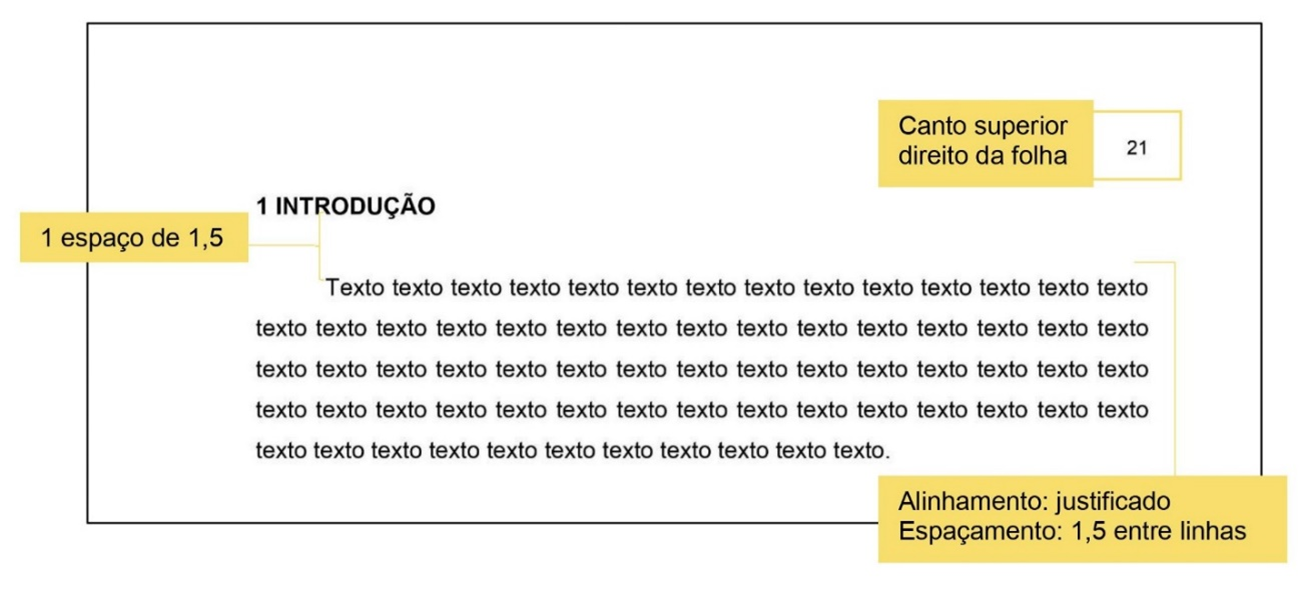
\includegraphics[scale=1]{Textuais/Picture1.png}
	\fonte{Elaborada pelos autores (2020), com base na NBR 14724 (2011).}
\end{figure}


\subsubsubsection{Seção quinaria}



O vídeo fornece uma maneira poderosa de ajudá-lo a provar seu argumento. Ao clicar em Vídeo Online, você pode colar o código de inserção do vídeo que deseja adicionar. Você também pode digitar uma palavra-chave para pesquisar online o vídeo mais adequado ao seu documento. Para dar ao documento uma aparência profissional, o Word\footnote{O Microsoft Word é um processador de texto produzido pela Microsoft Office foi criado por Richard Brodie para computadores IBM PC com o sistema operacional DOS em 1983.} fornece designs de cabeçalho, rodapé, folha de rosto e caixa de texto que se complementam entre si. Por exemplo, você pode adicionar uma folha de rosto, um cabeçalho e uma barra lateral correspondentes.

\begin{table}[!htbp]
	\centering
	%	\small
	\renewcommand{\arraystretch}{1.1}
	\caption{Modelo de tabela.}%
	\label{tab:tabela_exemplo}
	\begin{tabular}{ L{4cm}  R{3cm} || L{4cm}  R{3cm}  }
		\hline
		Município		& População Estimada & Município		& População Estimada 		\\ 
		\hline
		Abdon Batista		& 2630	& Bom Jesus				& 2821 \\ 
		Abelardo Luz		& 17717	& Bom Jesus do Oeste	& 2156 \\ 
		Agrolândia			& 10272	& Bom Retiro			& 9598 \\ 
		Agronômica			& 5306	& Bombinhas				& 17477 \\ 
		Água Doce			& 7132	& Botuverá				& 4943 \\ 
		Águas de Chapecó	& 6379	& Braço do Norte		& 31765 \\ 
		\hline
	\end{tabular}
	\vspace{2mm}
	\fonte{Adaptado de IBGE (2015).}
\end{table}

Clique em Inserir e escolha os elementos desejados nas diferentes galerias.

\begin{figure}
	\centering
	\caption{População.}
	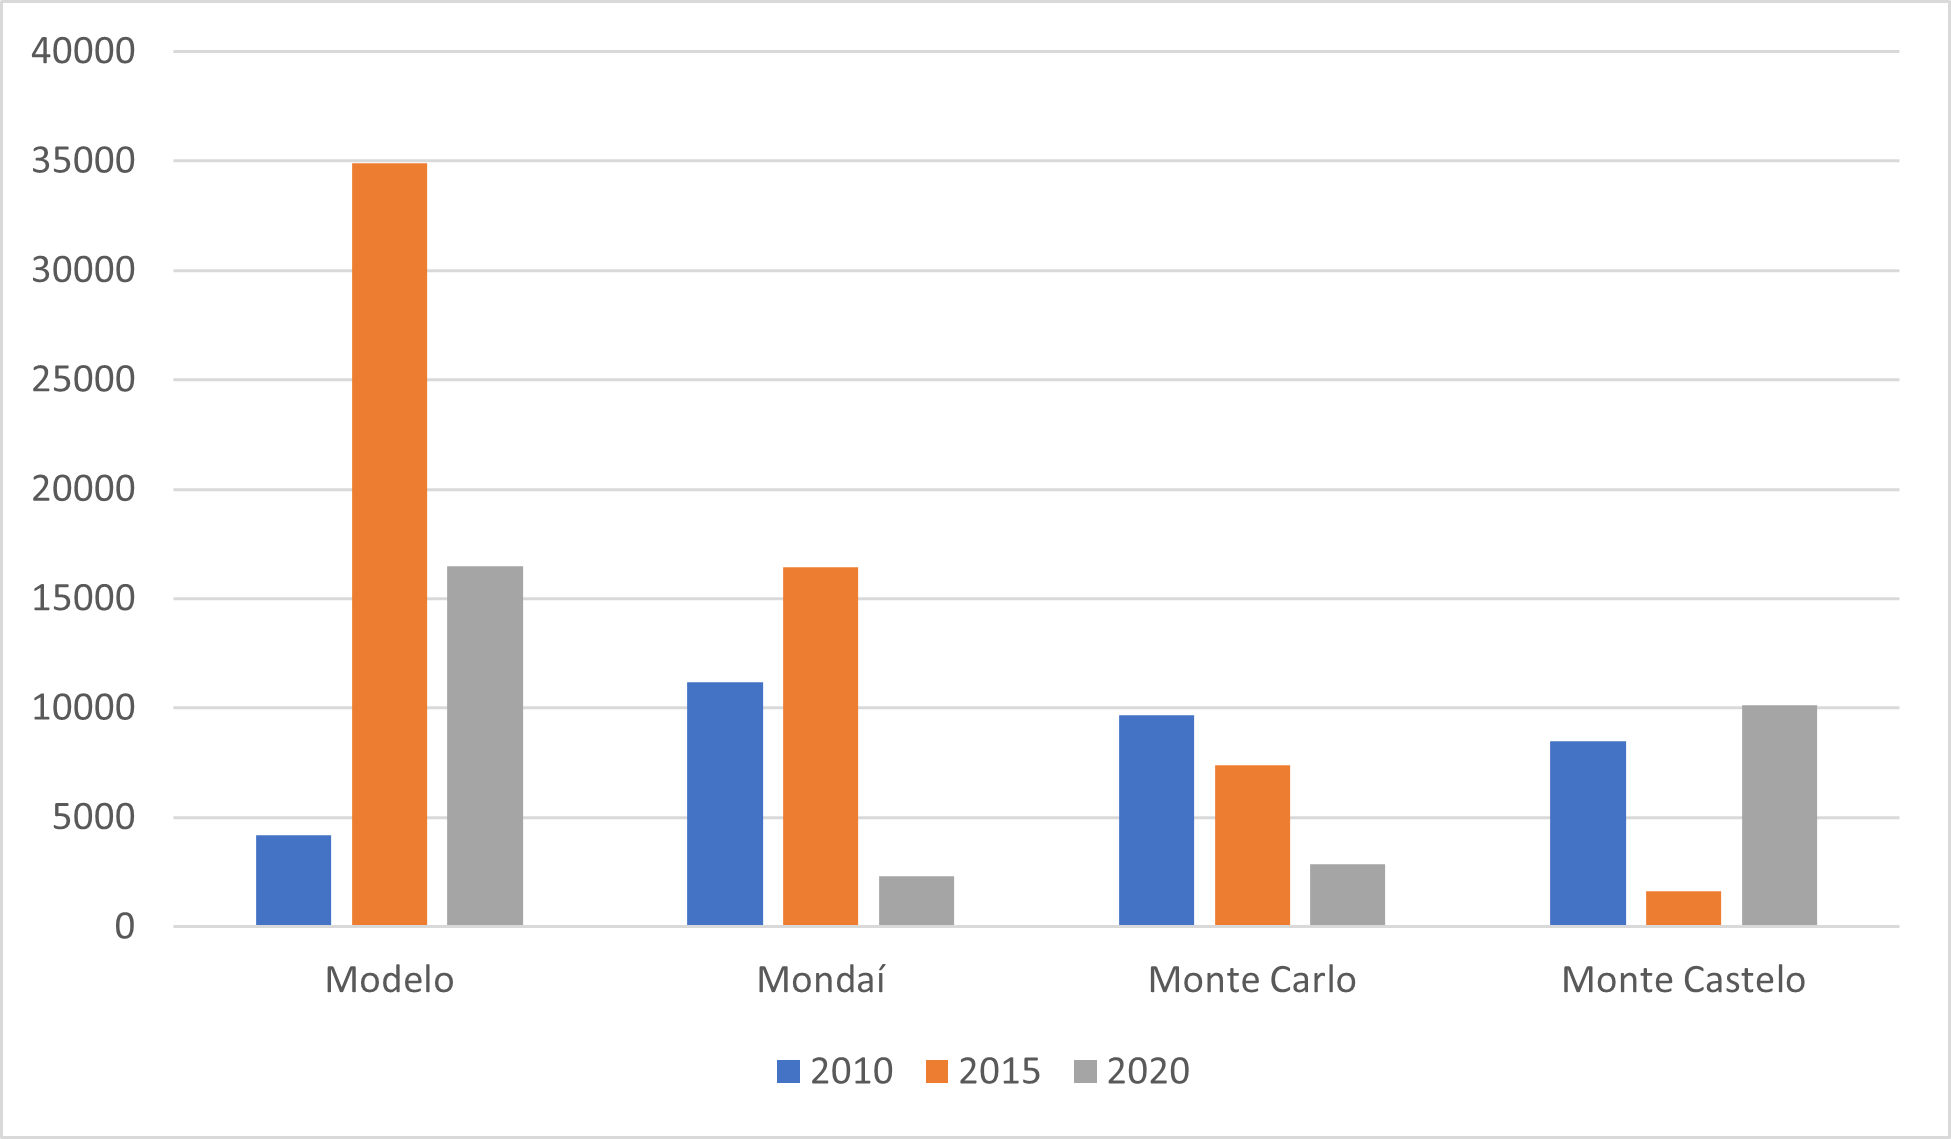
\includegraphics[scale=1]{Textuais/Picture2.png}
	\fonte{\me{2020}}
\end{figure}

As chamadas às equações e fórmulas, no texto, devem ser feitas da seguinte forma: equação (1), fórmula (2).

\textbf{Exemplo 1:}
O Teorema de Pitágoras, é uma equação \eqref{eq:eq1} que pode ser aplicada em qualquer triângulo retângulo (triângulo que tem um ângulo de 90°).
\begin{equation} \label{eq:eq1}
a^2 + b^2 = c^2 
\end{equation}

\textbf{Exemplo 2:}
A dopamina é um composto orgânico de função mista álcool, fenol e amina que apresenta fórmula \eqref{eq:form1} molecular:
\begin{equation} \label{eq:form1}
\ch{C8 + H11NO2} 
\end{equation}

\textbf{Exemplo 3:}
O modelo matemático de Huang (HUG), dado pelas equações \eqref{eq:eq3} e \eqref{eq:eq4}, foi elaborado com o intuito de fornecer uma descrição mais simples do crescimento bacteriano.
\begin{gather} 
	y(t) = y_0 + y_{max} -\ln{[e^{y_0}  + (e^{y_{max}} -e^{y_0} )  e^{-u_{max}\beta(t)} ]}   \label{eq:eq3}  \\
	\beta(t) = t + \frac{1}{4}\ln\left( \frac{1+ e^{-4(t-\lambda)} }{1+ e^{4(\lambda)} }\right) \label{eq:eq4}
\end{gather}
\noindent onde $y(t)$ corresponde ao logaritmo natural da concentração celular (log UFC/g) no instante $t$ (dias), $y_{max}$ é o logaritmo natural da população bacteriana (log UFC/g) final, $y_0$ corresponde ao logaritmo natural da população bacteriana inicial (log UFC/g) e $\beta(t)$ é a função de transição.

\textbf{Exemplo 4:}
Para o cálculo da intensidade fórmula \eqref{eq:eq5} de Intensidade-Duração-Frequência apresentada, os valores encontrados seguindo os parâmetros apresentados e como o resultado é dado em mm/h haverá também a sua conversão para m/s.
\begin{gather} 
	i = \frac{K T^m}{(t+b)^n}   \label{eq:eq5}  \\[2ex]
		i = \frac{\num{625.58} \cdot 5^{\num{0.171}}  }{(60+\num{8.89})^{\num{0.961}}} \\[2ex]
		i = \num{44.222} \cdot \frac{\si{mm}}{\si{h}} \cdot \frac{1\mathrm{m}}{\SI{1000}{mm}} \cdot \frac{\SI{1}{h}}{\SI{3600}{s}} 	
\end{gather}
\noindent onde, $i$ é a intensidade média máxima de precipitação, em mm/h; $T$ é o Período de retorno, em anos; $t$ é a duração da chuva, em minutos; $k,m,b,n$ são os parâmetros da equação determinados para cada local.


As citações diretas com até três linhas ``[...] devem estar contidas entre aspas duplas. As aspas simples são utilizadas para indicar citação no interior da citação.'' (ABNT, 2002, p. 2). Devem apresentar autor, ano e página. Quando a indicação de autor estiver dentro de parênteses, o sobrenome deve ser em letra maiúscula. 


As citações diretas com mais três linhas ``[...] devem ser destacadas com recuo de 4 cm da margem esquerda, com letra menor que a do texto utilizado e sem as aspas.'' (ABNT, 2002, p. 2). Ou seja, utilizar fonte tamanho 10 para as citações diretas longas, com espaçamentos simples entre linhas. As citações devem ser precedidas e antecedidas por um (1) espaço de 1,5 entrelinhas. 

\begin{citacao}
Texto texto texto texto texto texto texto texto texto texto texto texto texto texto texto texto texto texto texto texto texto texto texto texto texto texto texto texto texto texto texto texto texto texto texto texto texto texto texto texto texto texto texto texto texto texto. (SILVA, 2020, p. 21).
\end{citacao}


Nas citações indiretas não há necessidade de usar aspas e indicar a página, considerando que é uma paráfrase. Faz-se necessário apresentar o autor e ano.






\noindent Exemplo referência de livro: \cite{exemplo_livro}

\noindent Exemplo referência de livro em meio eletrônico: \cite{exemplo_livroe}

\noindent Exemplo referência de trabalho acadêmico (Dissertação de Mestrado): \cite{exemplo_dissertacao}

\noindent Exemplo referência de trabalho acadêmico (Tese de Doutorado): \cite{exemplo_tese}

\noindent Exemplo referência de artigo: \cite{exemplo_artigo}


\textbf{Para outras referências ver Manual Udesc}: \url{https://www.udesc.br/bu/manuais}









%


\chapter{Desenvolvimento}







%

\chapter{Conclusão}





% -----------------------------------------------------------------
% ELEMENTOS PÓS-TEXTUAIS
% -----------------------------------------------------------------
\postextual

% Você pode comentar os elementos que não deseja em seu trabalho;

% Referências bibliográficas
\bibliography{Referencias}	% Elemento Obrigatório

% ----------------------------------------------------------
% Glossário
% ----------------------------------------------------------

%Consulte o manual da classe abntex2 para orientações sobre o glossário.

%\glossary




% ----------------------------------------------------------
% Glossário (Formatado Manualmente)
% ----------------------------------------------------------

\chapter*{GLOSSÁRIO}
\addcontentsline{toc}{chapter}{GLOSSÁRIO}

{ \setlength{\parindent}{0pt} % ambiente sem indentação

\textbf{Ardósia}: Rocha metamórfica sílico-argilosa formada pela transformação da argila sob pressão e temperatura, endurecida em finas lamelas.

\textbf{Arenito}: rocha sedimentária de origem detrítica formada de grãos agregados por um cimento natural silicoso, calcário ou ferruginoso que comunica ao conjunto em geral qualidades de dureza e compactação.

\textbf{Feldspato}: grupo de silicatos de sódio, potássio, cálcio ou outros elementos que compreende dois subgrupos, os feldspatos alcalinos e os plagioclásios.






} % fim ambiente sem indentação


				% Elemento Opcional

% ----------------------------------------------------------
% Apêndices
% ----------------------------------------------------------

% ---
% Inicia os apêndices
% ---
\begin{apendicesenv}

% Imprime uma página indicando o início dos apêndices
%\partapendices

% ----------------------------------------------------------
\chapter{TÍTULO}
% ----------------------------------------------------------


\end{apendicesenv}
% ---				% Elemento Opcional

% ----------------------------------------------------------
% Anexos
% ----------------------------------------------------------
%
% ---
% Inicia os anexos
% ---
\begin{anexosenv}

% Imprime uma página indicando o início dos anexos
%\partanexos

% ---
\chapter{TÍTULO}
% ---



\end{anexosenv}
				% Elemento Opcional

%%---------------------------------------------------------------------
%% INDICE REMISSIVO
%%---------------------------------------------------------------------

\phantompart
\printindex

		% Elemento Opcional

\end{document}

% -----------------------------------------------------------------
% Fim do Documento
% -----------------------------------------------------------------	